% Chapter 3

\chapter{Methodology} % Main chapter title

\label{Chapter3} % For referencing the chapter elsewhere, use \ref{Chapter3} 

\lhead{Chapter 3. \emph{Methodology}} % This is for the header on each page - perhaps a shortened title

%----------------------------------------------------------------------------------------

	In this section, the adopted activity recognition pipeline from \cite{twinanda2015data} and the proposed voting scheme are explained in detail with various classification strategies.

%----------------------------------------------------------------------------------------

\section{Adopted Classification Pipeline \citep{twinanda2015data}}
\label{section:AdoptedClassificationPipeline}
The adopted pipeline \cite{twinanda2015data} is as follows: acquisition from a multi-view camera setup, interest point detection, feature extraction and building a data-driven non-rigid layout for feature encoding.

%----------------------------------------------------------------------------------------
\subsection{Multi-View RGBD Camera Setup}
\label{section:MultiViewRGBDCameraSetup}
    The proposed multi-view camera system contains two RGBD sensors, i.e. Asus XtionPro Live, mounted on the ceiling of the operating room. The cameras record both intensity and depth data synchronously at 14 fps with 640 x 480 resolution. While one of the sensors is capturing the area around the operating room bed, the other sensor captures the area with equipment table, in which large area of the operating rooms is covered.
    Furthermore, thanks to minimal overlapping of the views of the sensors, interference of infrared patterns of depth sensors are very less. The intrinsic parameters for each camera are obtained by calibration with checkerboard pattern. The extrinsic parameters are obtained  by using laser pointer method described in \cite{7035826}. Both camera views are shown in \ref{fig:cameraViews}. Panoramic view of the operating room that is showing the camera setups is provided in Appendix~\ref{AppendixA}.
    
\begin{figure}
\centering
\subfigure[Camera view 1 - intensity data]{\label{sfig:view1Intensity}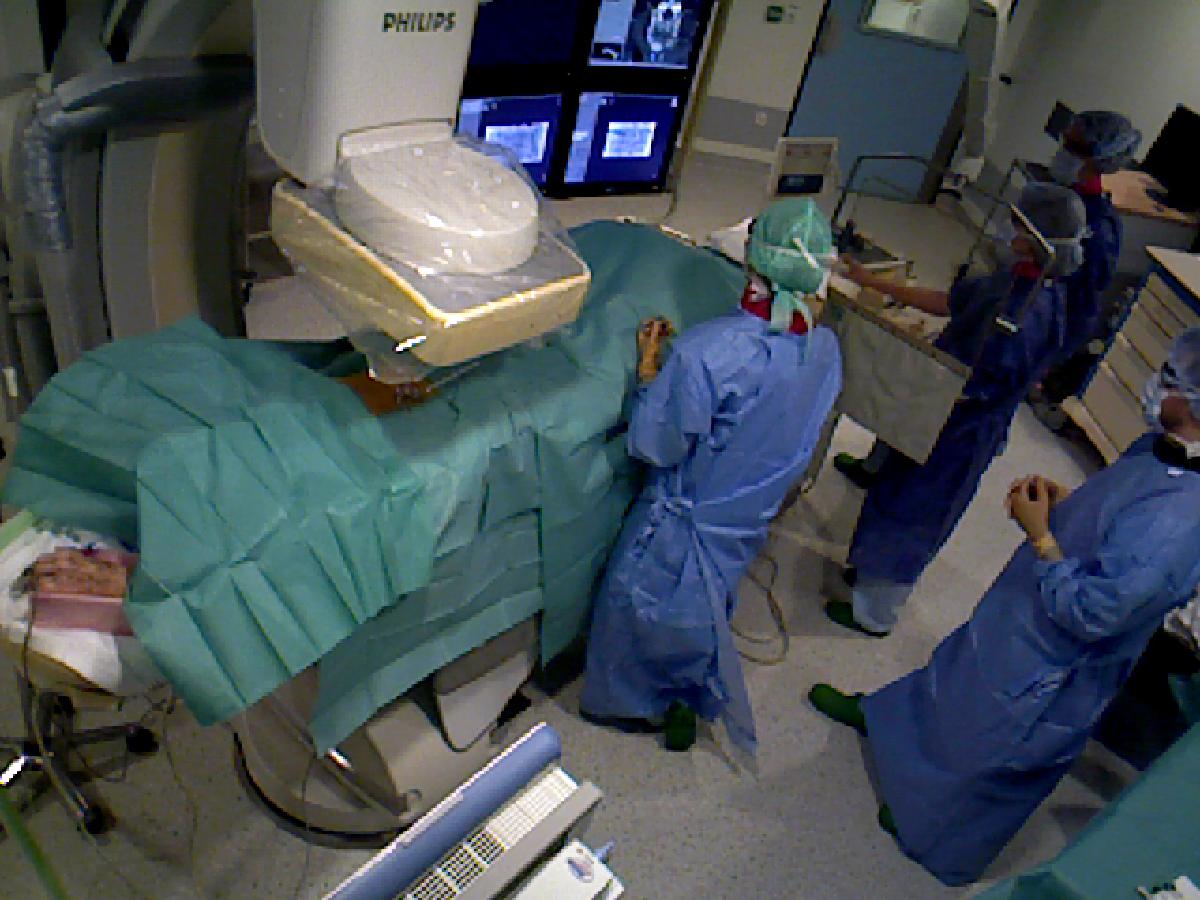
\includegraphics[width=.5\textwidth]{Figures/View1Color}}\hfill
\subfigure[Camera view 1 - depth data] {\label{sfig:view1Depth}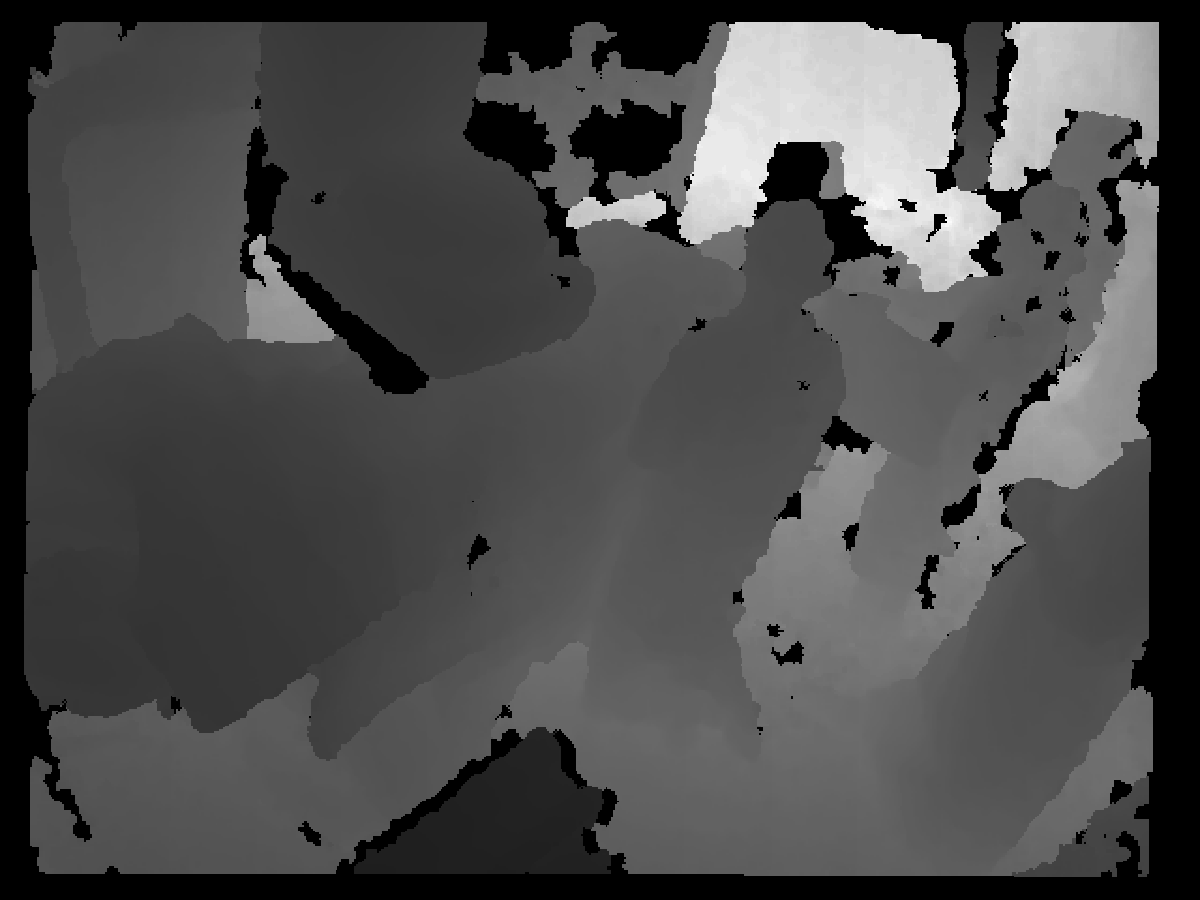
\includegraphics[width=.5\textwidth]{Figures/View1Depth}}\\
\subfigure[Camera view 2 - intensity data]{\label{sfig:view1Intesity}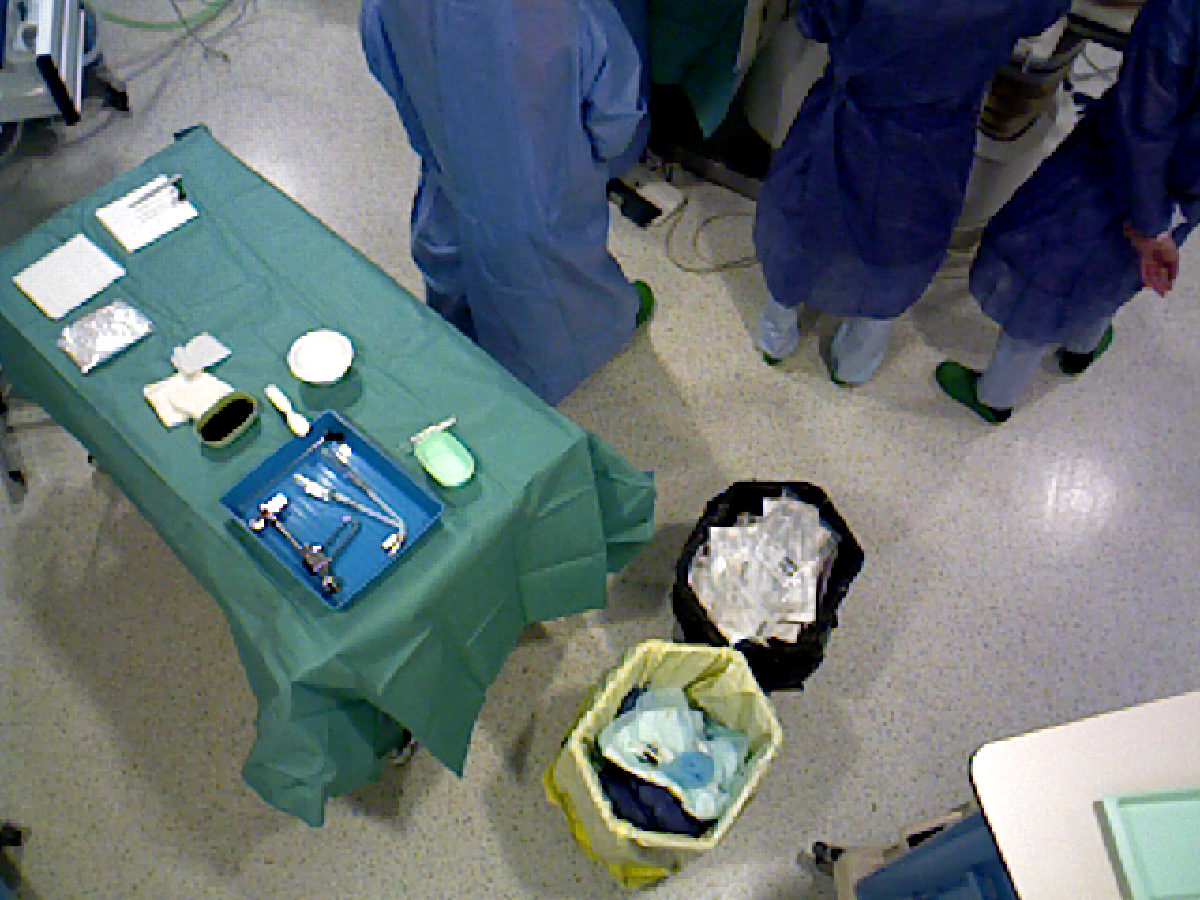
\includegraphics[width=.5\textwidth]{Figures/View2Color}}\hfill
\subfigure[Camera view 2 - depth data]{\label{sfig:view2Depth}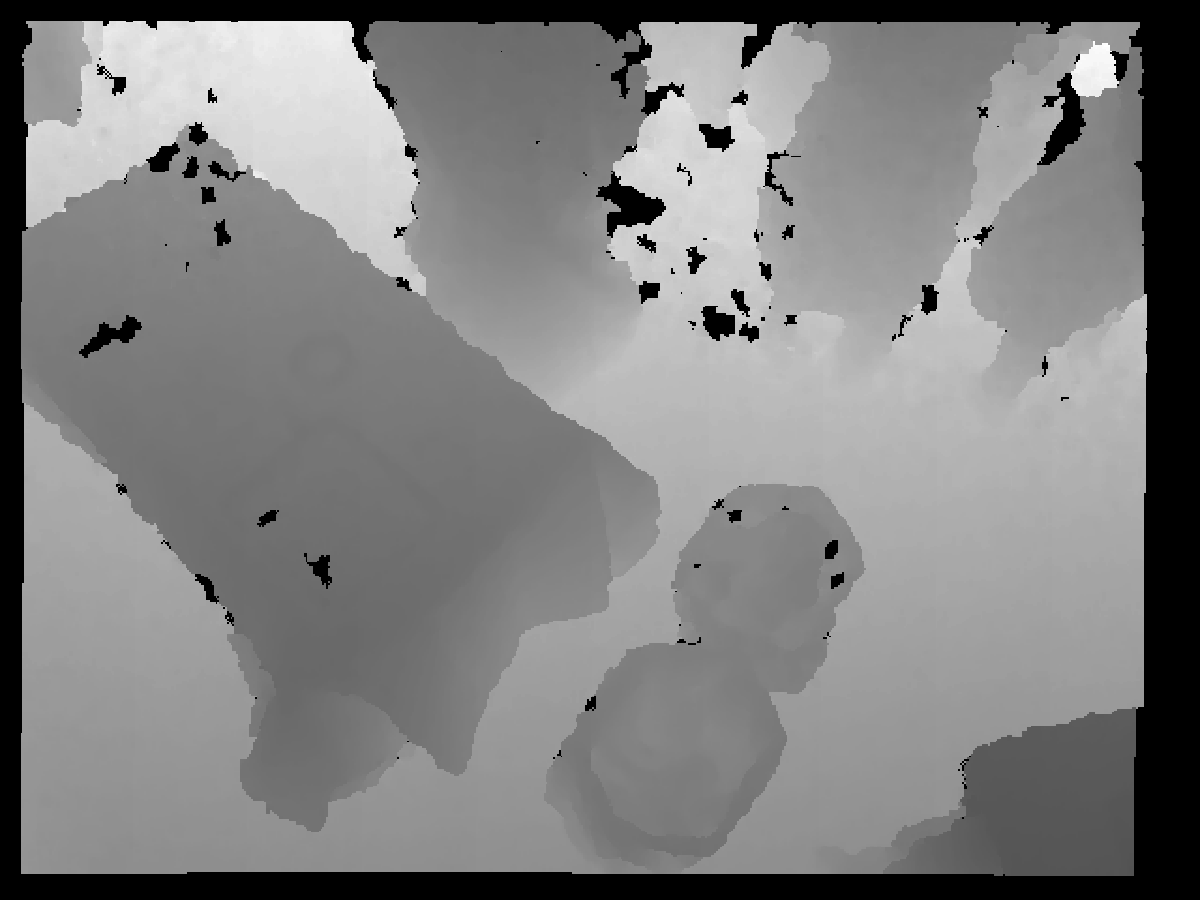
\includegraphics[width=.5\textwidth]{Figures/View2Depth}}\\
\caption{Sample images from RGBD sensors with view 1 and view 2.}
\label{fig:cameraViews}
\end{figure}
%----------------------------------------------------------------------------------------
\subsection{Interest Point Detection}
\label{section:InterestPointDetection}
	In the activity recognition pipeline, spatio-temporal interest points (STIP) by \citet{1570899} are used for intensity data. STIPs are computed by applying separable linear filters to get local maximum of the response. The response fuction $R$ of an intensity image $I$ is calculated as follows:

\begin{equation}
R_{I} = \left(I * g * h_{even}\right)^{2} + \left(I * g * h_{odd}\right)^{2},
\label{eq:stipResponseFunction}
%\nonumber
\end{equation}

	where $g(x, y; \sigma)$ is the 2D Gaussian smoothing kernel with scale $\sigma$, applied on the spatial $\left(x, y\right)$ dimensions. Terms $h_{even}$ and $h_{odd}$ are the quadrature pair of 1D Gabor filters applied in temporal domain defined as: $h_{even}\left(t|\tau,\omega,\right)=\cos\left(2\pi\omega t\right)e^{\frac{-t^{2}}{2\tau^{2}}}$ and $h_{odd}\left(t|\tau,\omega\right)=\sin\left(2\pi\omega t\right)e^{\frac{-t^{2}}{2\tau^{2}}}$.
    
    However, the STIP detector does not perform well and falsely detected on depth data because of the nature of the depth data where it may contain noise from sensors, pattern interference and fast foreground/background change of the border pixels. In order to cope with these problems, DSTIP detector by \citet{6619209} is used to detect depth spatio-temporal interest points (DSTIP) on depth data which introduced filtering method to reduce the noise and the false detection. Additional noise suppression term is proposed for noise filtering to equation \ref{eq:stipResponseFunction}:

\begin{equation}
R_{D} = \left(D * g * h_{even}\circ\bar{s}\right)^{2}+\left(D * g * h_{odd}\circ\bar{s}\right)^{2},
\label{eq:dstipResponseFunction}
%\nonumber
\end{equation}

where $D$ is the depth image, and $\bar{s}$ is the noise suppression term.


%----------------------------------------------------------------------------------------
\subsection{Feature Extraction}
\label{section:FeatureExtraction}
We compute features by extracting 3D cuboid around each detected interest points in spatio-temporal location $\left(x, y, t\right)$. Thus, the cuboids are the spatio-temporally windowed pixel values that contain most of the data contributed to response function \ref{eq:stipResponseFunction} and \ref{eq:dstipResponseFunction} to detect interest points. The size of the cuboids $\left(\Box_{x}\times\Box_{y}\times\Box_{t}\right)$ is proportionally assigned according to the spatial scale $\sigma$ and the temporal scale $\tau$.

Intensity cuboids are extracted from intensity data and histograms of optical flow (HOF) are calculated from the intensity cuboids. HOFs are used in intensity feature extraction process due to its distinguishable properties for direction of motion. These properties help to distinguish activities which have similar movements with different directions.

Moreover, 3D depth cuboids are extracted from depth data. Then, the depth cuboid similarity features (DCSF) \cite{6619209} are computed from the cuboids. DCSFs are computed based on self-similarity to encode spatio-temporal structure of the 3D cuboid. DCSF divides cuboids into smaller voxels, compute histograms of the depth pixels from each voxel, calculating relationship of each voxel by defining similarity between voxels using Bhattacharyya distance, then combination of all similarity scores from the voxels are concatenated to generate a DCSF feature.

%----------------------------------------------------------------------------------------
\subsection{Data Driven Feature Encoding}
\label{section:DataDrivenFeatureEncoding}

	The bag-of-words (BoW) is a model that treats image features as words to construct vocabulary. Then, histogram of occurrences of the words from the vocabulary produces a sparse histogram vector. $K$-means is typically used to encode the features which provide a global representation with BoW where $\mathbf{x}$ is a feature, $ \forall \mathbf{x} $, a value $w\in\left\{ 1,\cdots,K\right\}$, where $K$ is number of $K$-means center, is assigned to describe the index of the $K$-mean center which is the closest to feature $\mathbf{x}$. Hence $K$-means clusters every feature vector $\mathbf{x}\in\mathbb{R}^{n}$ and express them in a sparse representation $\mathbf{s}\in\mathbb{R}^{K}$ which is the occurrences of the words from the learnt dictionary $\mathbf{D}\in\mathbb{R}^{n\times K}$

	In \cite{twinanda2015data}, learning two separate dictionaries are proposed: a visual dictionary $\mathbf{D_{v}}$ with $K_{v}$ centers and a spatio-temporal dictionary $\mathbf{D_{st}}$ with $K_{st}$ centers. The visual dictionary $\mathbf{D_{v}}$ is learnt for encoding the visual features, i.e., the HOF and the DCSF for representing video clips. On the other hand, the spatio-temporal dictionary $\mathbf{D_{st}}$ is learnt by clustering the locations of the interest points $\left(x,y,z,t\right)$, where $X=\left(x,y,z\right)$
and $t$ are the 3D coordinates and the temporal location
of the interest point, respectively. Since the video clips varies in length, $t$ is normalized by length of its video clip. Multi-view camera systems require to define one camera's coordinate system as a reference coordinate system to transform the 3D coordinates into a common coordinate system. Hence, the final 3D coordinates are computed by:

\begin{equation}
\begin{array}{c}
X=T_{R}\cdot Y+T_{t}\\
Y=d\cdot C^{-1}\cdot\left(\begin{array}{ccc}
u & v & 1\end{array}\right)^{\top},
\end{array}
\end{equation}

where $Y$ is the 3D point in the camera frame, $\left(u,v\right)$
and $d$ are respectively the image pixel coordinates and the corresponding
depth value, $C$ is the intrinsic camera matrix, $T_{R}$
and $T_{t}$ are respectively the rotation and translation from the
camera frame to the reference frame. Then, learnt spatio-temporal dictionary $\mathbf{D_{st}}$ is used to place a non-rigid spatio-temporal grid to divide the spatio-temporal space into patches $\{P^{1},...,P^{K_{st}}\}$. These local patches from the non-rigid layout are high dimensional 4D patches. One example of feature encoding in 2D space is shown in Figure~\ref{fig:featureEncoding} where non-rigid layout is learnt by clustering points indicated with colored patches and features are extracted from the patches.

\begin{figure}[htbp]
\begin{center}
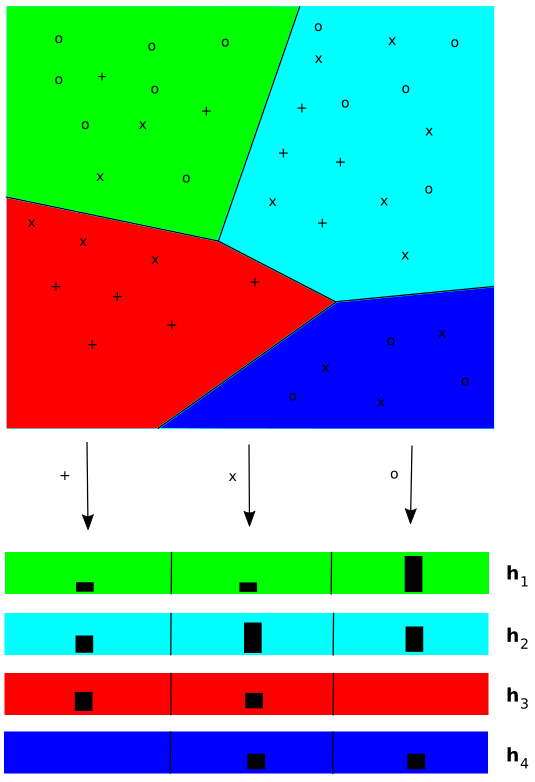
\includegraphics[scale=0.5]{Figures/featureEncoding}
\end{center}
\caption{Example of data driven feature encoding in 2D space with $K_{v}$ = 3 and $K_{st}$ = 4\label{fig:featureEncoding}}
\end{figure}
    
	In order to get the final histogram representation of the patches for a video clip $V_{i}$, where $i$ is video instance count, firstly, all features, $\forall \mathbf{x}$, belong to their corresponding patch, $P^{j}$, are found using the $\mathbf{D_{st}}$. Secondly, using the $\forall \mathbf{x} \in P^{j}$, the histogram of visual word occurrences from every patch $P^{j}$ is computed using $\mathbf{D_{v}}$. Finally, we obtain $K_{st}$ histograms, $\{_{i}H^{1},..., _{i}H^{K_{st}}\}$, representing the patches $P^{j}$ from video clip $V_{i}$, where $_{i}H^{j} \in \mathbb{R}^{K_{v}}$.
%----------------------------------------------------------------------------------------
\section{Voting Scheme}
\label{section:VotingScheme}
We extended the pipeline aforementioned by proposing a voting scheme. The proposed voting scheme uses histograms $H^{j}$ obtained from patches $P^{j}$ of a data-driven non-rigid layout presented in Section~\ref{section:DataDrivenFeatureEncoding}. We classify every local patch $P^{j}$ using $H^{j}$ independently and collect their vote for calculating majority vote for global activity. Hence every patch $P^{j}$ holds information about activity with semantic information that is contributing globally. 

%----------------------------------------------------------------------------------------
\section{Activity Classification}
\label{section:ActionClassification}

	In our multi-view camera system, every activity $a_{i}$ is recorded from both of the views. Hence, it produces a video clip pair $\left(V_{i}^{1},V_{i}^{2}\right)$ from the cameras. Firstly, interest point detection in Section~\ref{section:InterestPointDetection} is applied on the video clip pair $\left(V_{i}^{1},V_{i}^{2}\right)$ and features are extracted as described in Section~\ref{section:FeatureExtraction}. Then, two dictionaries are learnt for encoding as described in Section~\ref{section:DataDrivenFeatureEncoding}. The learnt spatio-temporal dictionary divides 4D space into smaller local 4D patches $\{P^{1},...,P^{K_{st}}\}$. Then, histogram representation $H^{j}$ from each local patch $P^{j}$ is calculated using the learnt visual dictionary for the video clip pair $\left(V_{i}^{1}, V_{i}^{2}\right)$. In order to get final histogram representation, $\{_{i}H^{1},..., _{i}H^{K_{st}}\}$, for video clip pair $\left(V_{i}^{1},V_{i}^{2}\right)$, we merge information by computing $_{i}H^{j} = _{i}^{1}H^{j} + _{i}^{2}H^{j}$ where $_{i}^{1}H^{j}$ and $_{i}^{2}H^{j}$ are respectively histograms from patch $P^{j}$ of $V_{i}^{1}$ and $V_{i}^{2}$. Then, final histograms, $\{H^{1},..., H^{K_{st}}\}$ from all video clip pairs are passed to the classifier for training and testing. In order to make performance comparison, we use the one-against all Support Vector Machine (SVM) with the nonlinear kernel, and we use Random Forest implementation to give comprehensive comparison of the voting scheme.

\subsection{SVM}
\label{section:SVM}
Support Vector Machine (SVM) is a well known supervised machine learning model for classification and regression. It uses hyper-planes in high dimensional space to divide training data with largest margin of the points. In this work, non-linear SVM with Chi-square $ \left(\mathcal{X}\right)^{2} $ and histogram intersection kernel is used. Since we have multi-class problem, we use one-against-all SVM to handle multi-class problem.



\subsection{Random Forest}
\label{section:RandomForest}
Random Forest is an algorithm of ensemble learning methods that used for classification and other tasks. Random Forest is collection of multiple decision trees that each produces a probabilistic response of the prediction of the classes with bagging and random selection of features. Then, these responses are combined to construct prediction which reduces over-fitting problem of the single decision tree models. Random Forest can be thought as a group of weak learners combined to get stronger learner.



\subsection{Training Strategy}
\label{section:TrainingStrategy}
In this work, we propose to use a two-level classification strategy to carry on the voting scheme. In the first level, we learn a classification model to obtain the probability votes from the 4D patches. However, in the second level classification, we learn the weights for the probability votes under the assumption that each patch has different contribution. In addition to the proposed training strategy, we also propose to use two different approaches used in the first level of the proposed classification strategy, i.e., one-model and multi-model approaches. In the one-model approach, all histograms from each patch from each video is trained using one classifier. However, in the multi-model approach, separate classifiers are trained for each patch.

\subsubsection{One-Model Approach}
\label{section:OneModelApproach}
In one-model approach, we use one classifier model in each level, i.e., $M_{level1}$ and $M_{level2}$. First, we train $M_{level1}$ with the training set which consists of a collection of histogram vectors $\{H^{1}, ..., H^{K_{st}}\}$. Then, we pass the histogram vectors to $M_{level1}$ to get the probability votes $\{W^{1}, ..., W^{K_{st}}\}$ from each video clip pair where $W^{j} \in \mathbb{R}^{N_{c}}$ and $N_{c}$ is the number of activity classes. Then, we concatenate the probability vectors, $W = \left[(W^{1})^{T}, ..., (W^{K_{st}})^{T}\right]^{T}$ where $W \in \mathbb{R}^{N_{c} \cdot K_{st}}$, of the same video clip. Finally, we train the second level classifier model $M_{level2}$ with the concatenated probability vectors $W$. Testing is done with same order: (1) testing set is passed through the first level classifier model $M_{level1}$ and the probability votes from the same video clips are concatenated, (2) concatenated probability votes are passed through the second level model $M_{level2}$ to to get the final classification probability. An illustration of the one-model approach is shown in Figure~\ref{fig:oneModelApproachIllustration}.
    
\begin{figure}[!htbp]
\begin{center}
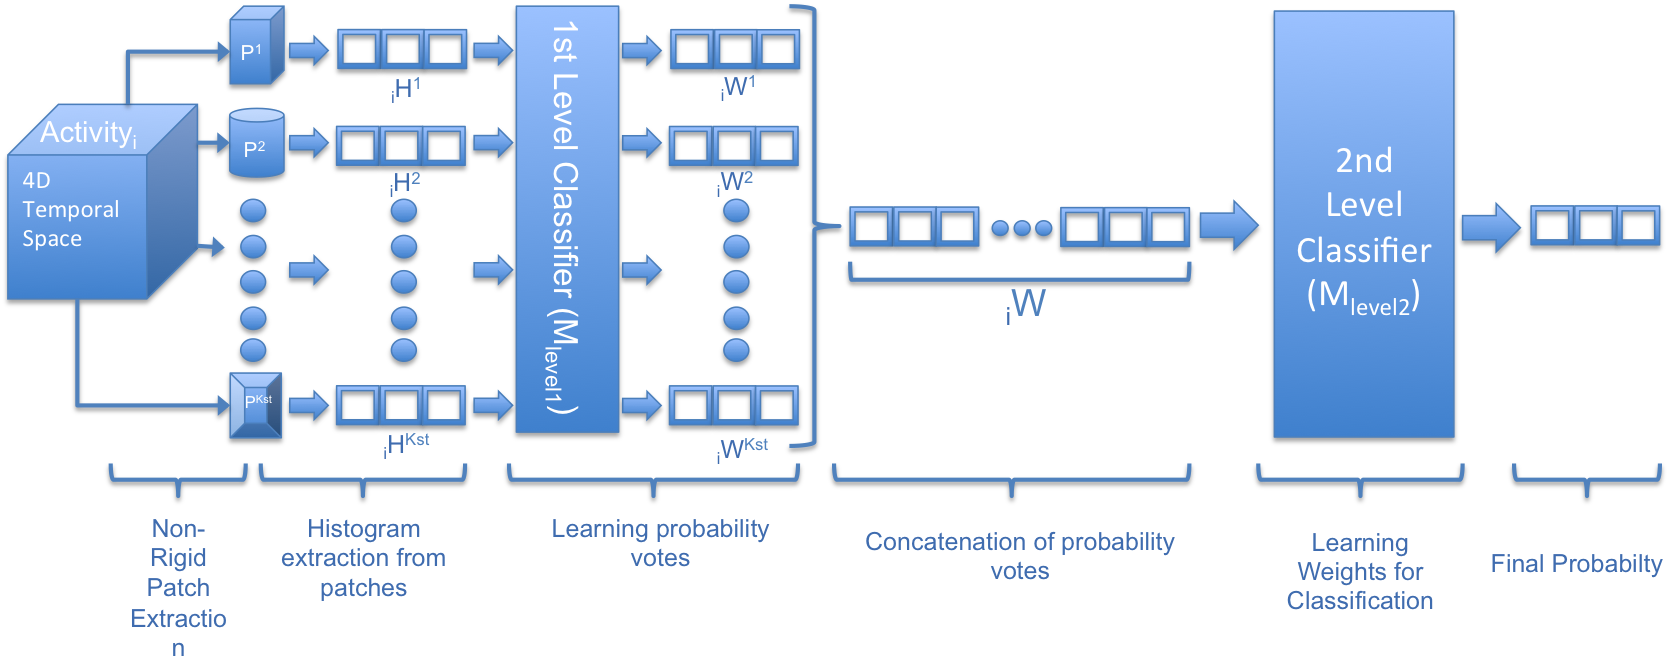
\includegraphics[scale=0.50]{Figures/oneModelApproach3}
\end{center}
\caption{Illustration of one-model approach to classify a video clip \label{fig:oneModelApproachIllustration}}
\end{figure}


\subsubsection{Multi-Model Approach}
\label{section:MultiModelApproach}
In contrast to the one-model approach, we propose to use multiple classifiers in the first level classification. Each patch $P^{j}$ in the first level classification has its own classifier model, i.e., $\{M_{level1}^{1},\dots,M_{level1}^{K_{st}}\}$. In order to train the first level classifiers, $\{M_{level1}^{1},\dots,M_{level1}^{K_{st}}\}$, the training set is separated into $K_{st}$ for each patch type. Each first level classifier, $M_{level1}^{j}$, is trained with its corresponding patch histograms, i.e., $\{_{1}H^{j},...,_{N_{v}}H^{j}\}$ where $N_{v}$ is number of video clip pairs. Then, we use the same training set to test the models to get probability votes, $\{W^{1},...,W^{K_{st}}\}$ where $W^{j} \in \mathbb{R}^{N_{c}}$ and $N_{c}$ is the number of activity classes. Then, we get concatenated probability vector $W$ for each video clip as described in Section~\ref{section:OneModelApproach} and train the second level classifier. Testing is done as follows: (1) testing set is separated according to patch types, (2) each patch type is tested though the corresponding classifier in the first level to get probability votes, (3) histograms from the first level is concatenated and tested against the second level. An illustration of the multi-model approach is shown in Figure~\ref{fig:multiModelApproachIllustration}.
    
    
\begin{figure}[!htbp]
\begin{center}
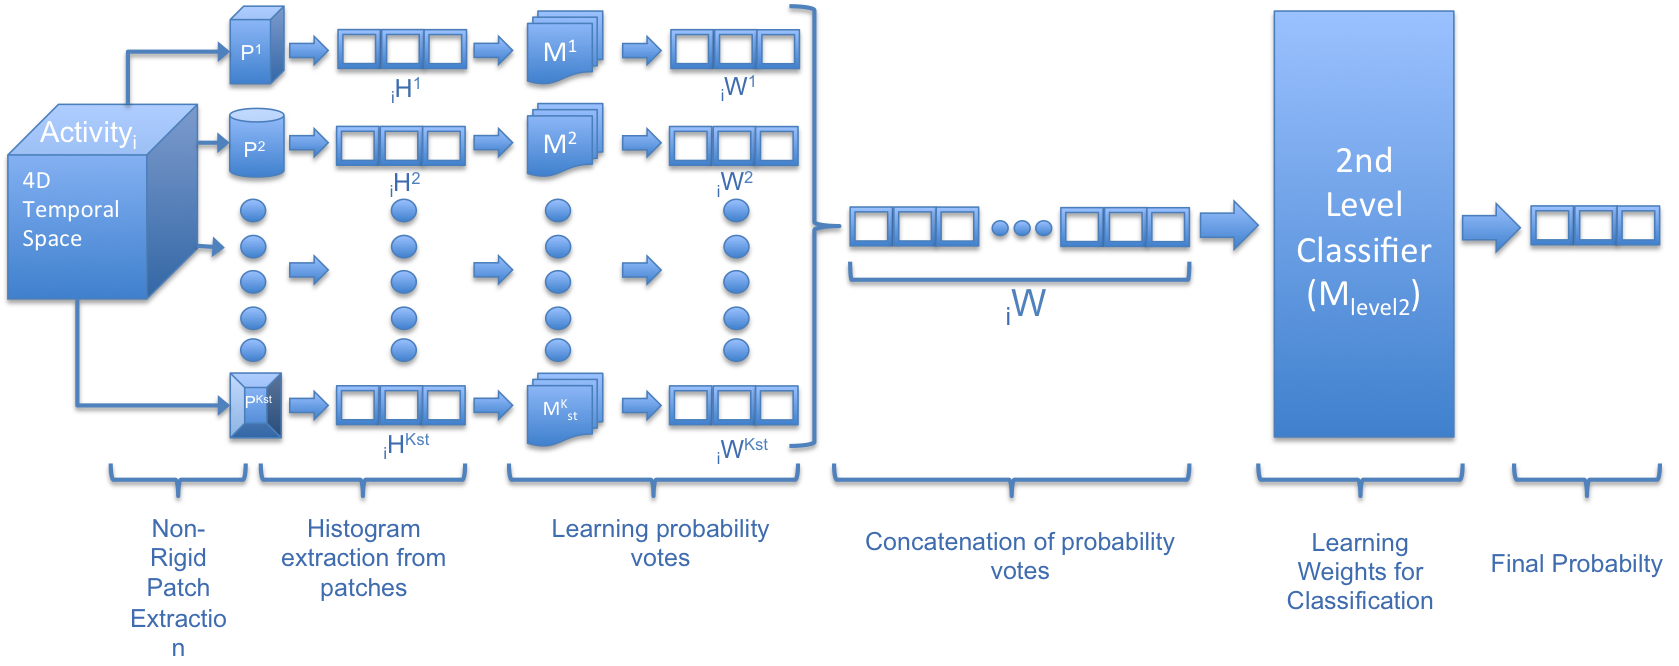
\includegraphics[scale=0.5]{Figures/multiModelApproach3}
\end{center}
\caption{Illustration of multi-model approach to classify a video clip \label{fig:multiModelApproachIllustration}}
\end{figure}




























